\chapter{Out-Of-Core-Ansatz}

Out-of-Core-Strategien erm�glichen einer Anwendung oder einem System die Verwendung von Datenmengen, welche die lokale Speicherkapazit�t �bersteigen. Voraussetzung daf�r ist die Segmentierbarkeit der Daten. Ausserdem muss die lokal gespeicherte Untermenge der segmentierten Daten zu jedem Zeitpunkt zur Verarbeitung gen�gen.
\begin{figure}[position=h]
  \centering
  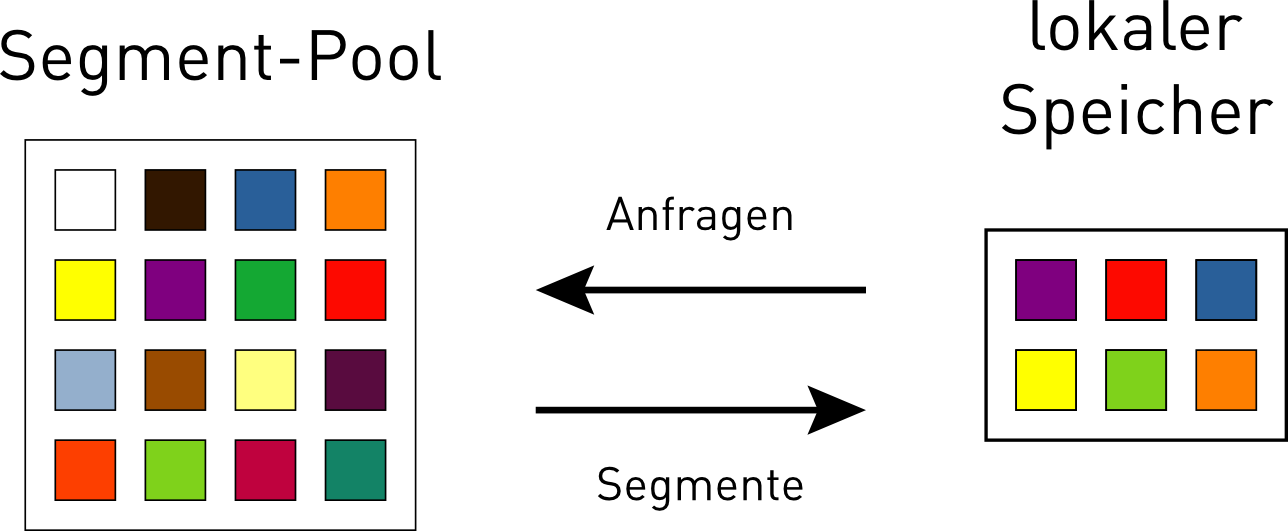
\includegraphics[width=0.75\textwidth]{out-of-core-ansatz/figures/out_of_core_pricipe.png}
  \caption{Out-Of-Core-Prinzip\label{out_of_core_pricipe}}
\end{figure}
\\
Die endliche Menge lokalen Speichers der GPU begrenzt die maximale Aufl�sungen der SVO-Struktur. Eine Vergr��erung des Speichers l�st das Problem nicht da wie oben beschrieben eine weitere SVO-Tiefe etwa die vierfache Speicher\-menge ben�tigt.


% /////////////////////////////////////////////////////////////////////////////


\section{Segmentierung}

Die Unterteilung der SVO-Struktur erfolgt in Unterb�umen fester Gr��e die in dieser Arbeit als \textit{Treelets} (B�umchen) bezeichnet werden. (!!! etwas �ber die Gr��e der Treelets sagen) Ein Treelet hat eine eindeutige Kennung (\textit{Treelet-Id}) und h�lt unter Anderem Informationen �ber sein �bergeordnetes Treelet und seine untergeordneten Treeles wodurch eine zus�tzliche, bidirektionale Baumstruktur �ber dem eigentlichen Octree entsteht. Dabei entspricht jeder Blattknoten eines Eltern-Treelets dem Wurzelknoten eines Kind-Treelets.
\begin{figure}[position=h]
  \centering
  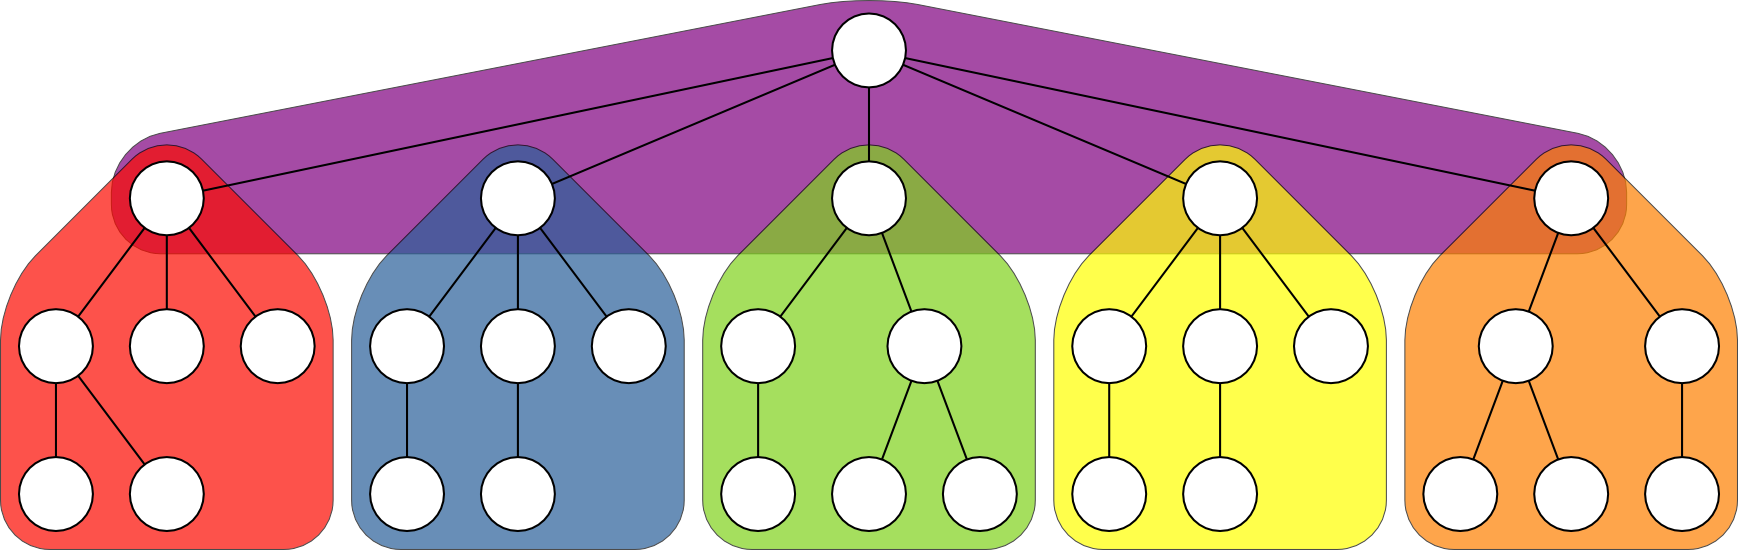
\includegraphics[width=0.75\textwidth]{out-of-core-ansatz/figures/fixed_size_treelets.png}
  \caption{Treelet-Struktur mit 6 Knoten pro Treelet \label{fixed_size_treelets}}
\end{figure}
\\
Die Verbindung zum �bergeordneten Treelet (\textit{Eltern-Treelet}) ist wichtig, da aufgrund der zugrundeliegenden Baumstruktur die Verarbeitung eines Treelets das Vorhandensein des Eltern-Treelets voraussetzt. In jedem Treelet ist die Position des entsprechenden Blattknotens im Eltern-Treelet und die Position dessen Elternknoten gespeichert. Die Verbindungen nach unten sind im Erstes-Kind-Index der Blattknoten gespeichert, sind damit Teil der SVO-Daten und somit f�r alle Operationen auf auf dem SVO verf�gbar.\\

!!!
- Gr��e eines Treelets -> Anzahl von Knoten Beispiel
- Verweis zu Untergeordneten Treelets in Blattknoten FirstChildIndex
 

% /////////////////////////////////////////////////////////////////////////////


\section{Prinzipieller Aufbau}

Der in dieser Arbeit verwendete Out-Of-Core-Ansatz besteht grunds�tzlich aus vier Teilen (Abbildung \ref{four_part_setup}): Einem gro�en, clientseitigem Buffer der die gesammte SVO-Struktur h�lt, einem vergleichsweise kleinen, serverseitigen Buffer der eine Untermenge der SVO-Struktur halten kann (\textbf{\textit{Incore-Buffer}}), einer Speicherverwaltung die den serverseitigen Buffer pflegt und einem Analysesystem das entscheidet welche Teile serverseitig ben�tigt werden.
\begin{figure}[position=h]
  \centering
  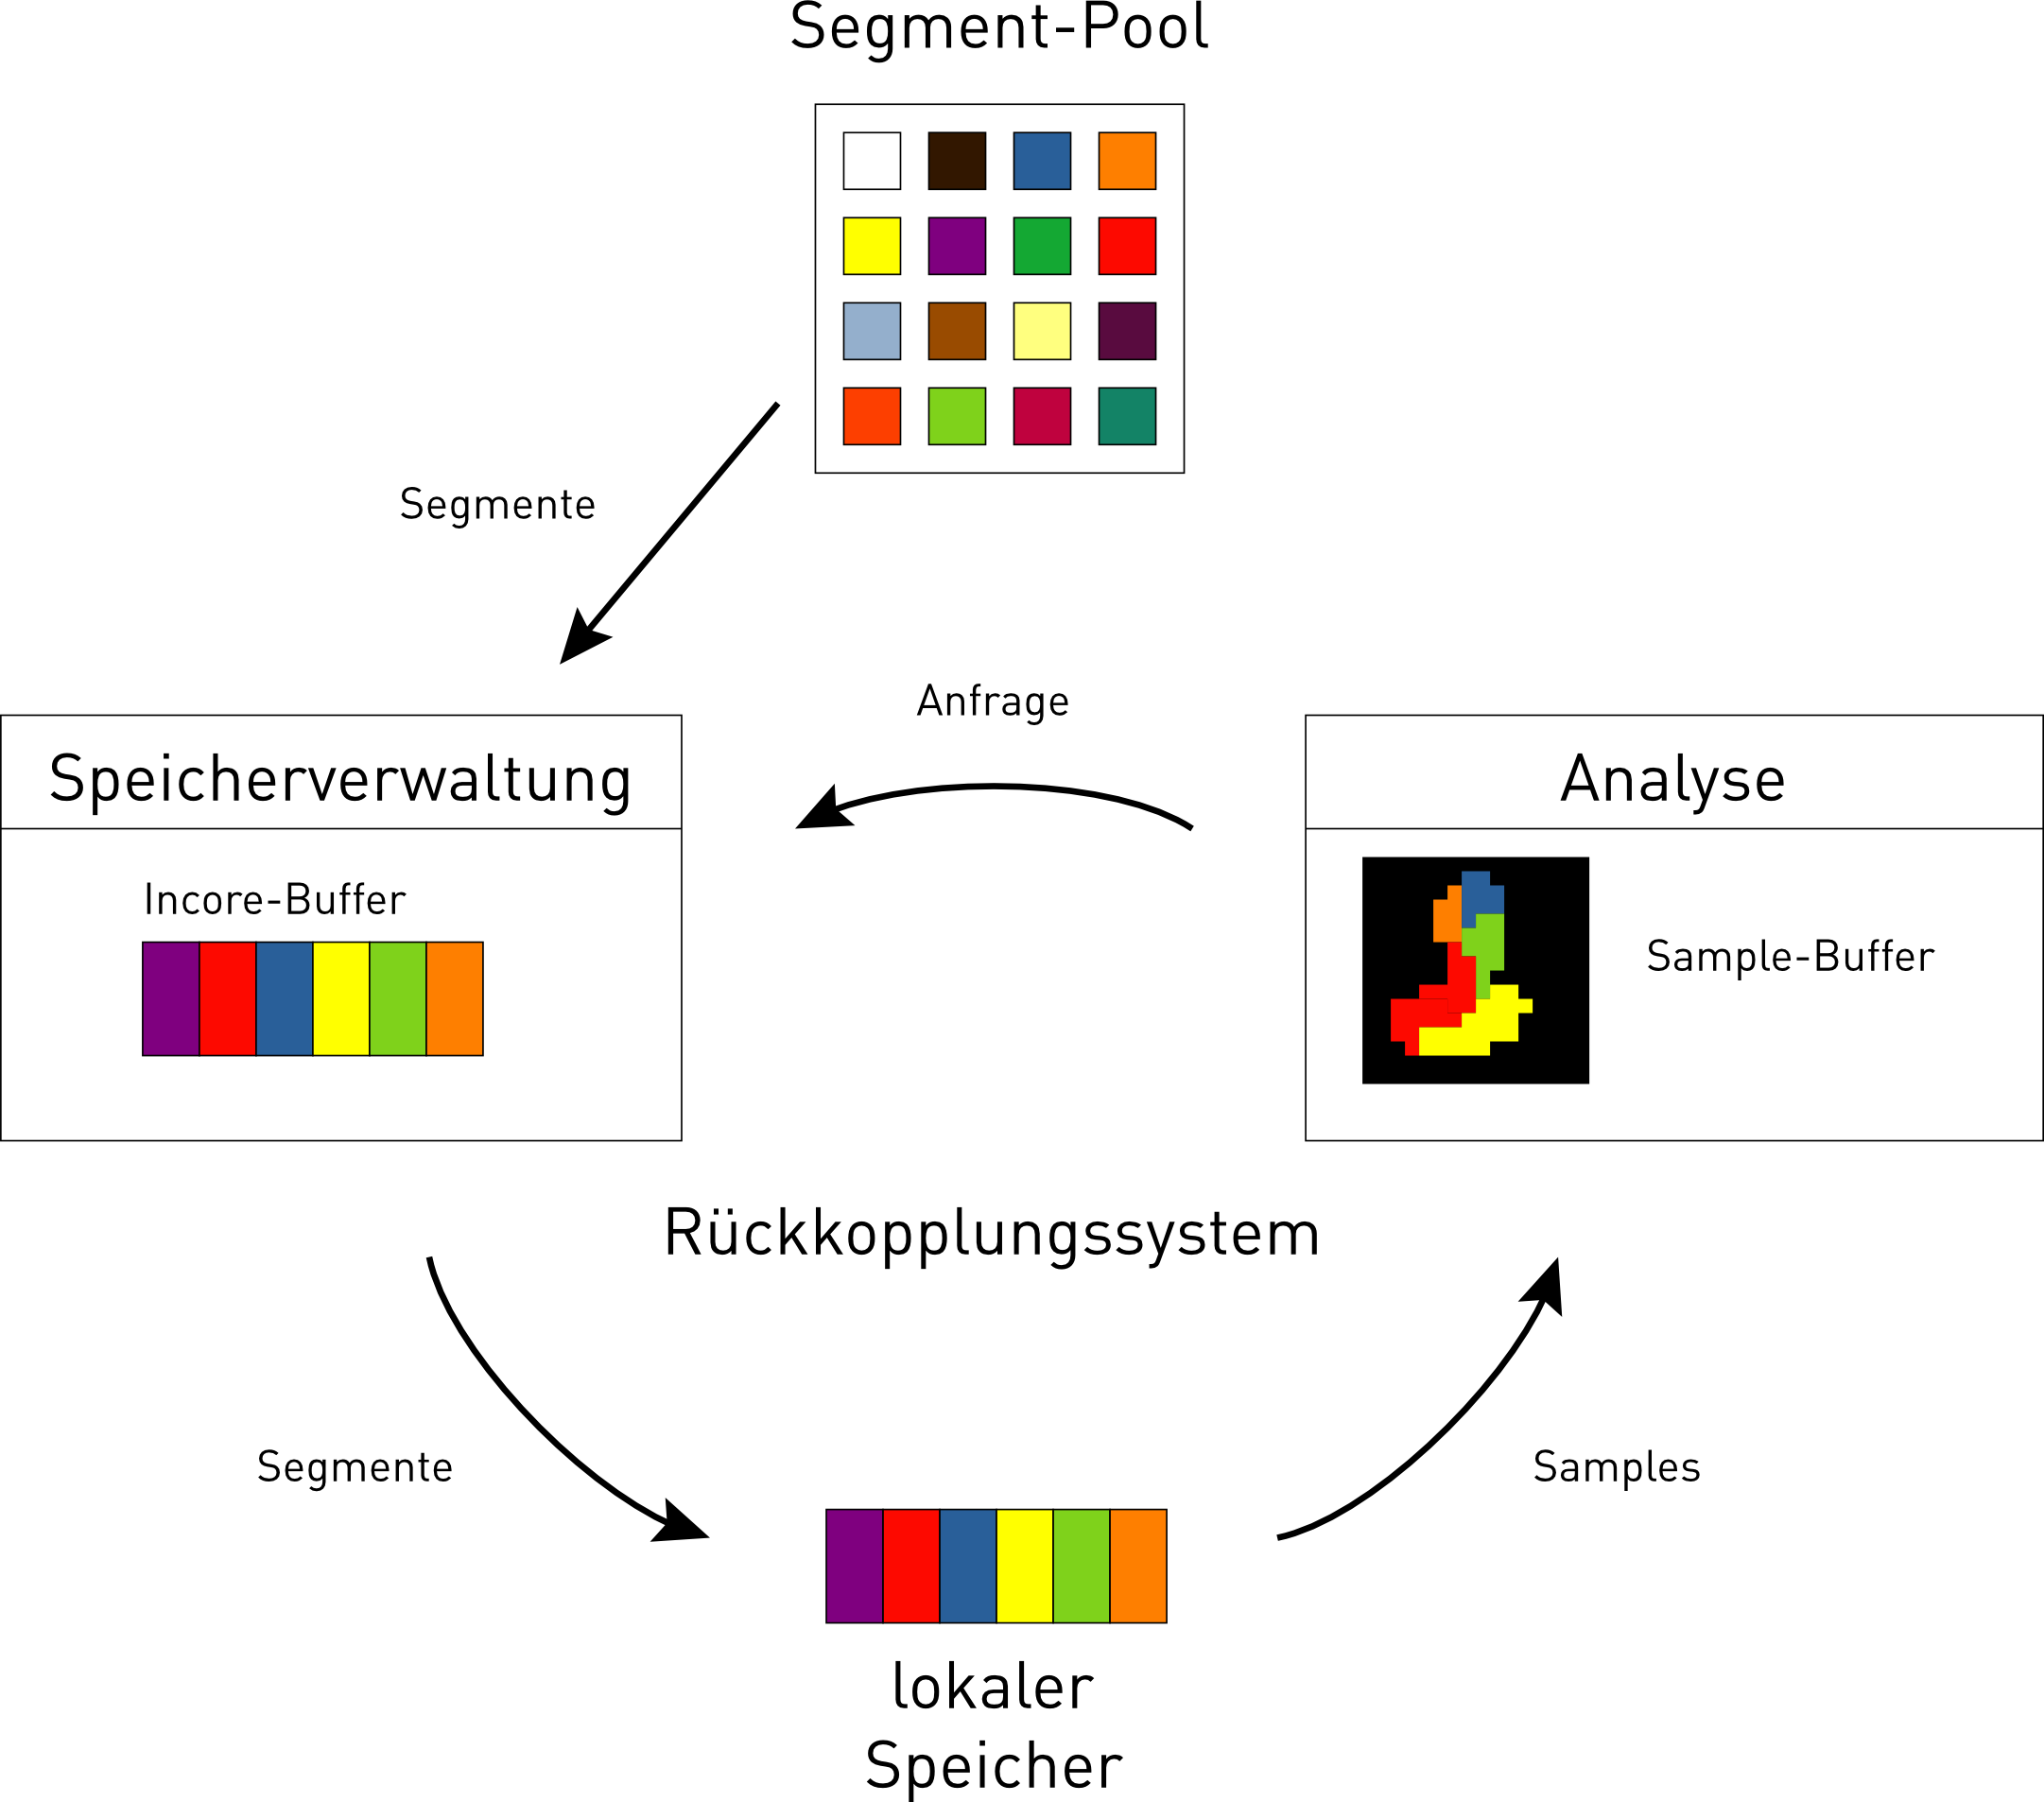
\includegraphics[width=0.75\textwidth]{out-of-core-ansatz/figures/four_part_setup.png}
  \caption{Aufbau des Out-Of-Core-Systems\label{four_part_setup}}
\end{figure}
\\
Der Incore-Buffer, der auf Client- und Serverseite Vorhanden ist, wird wie der SVO in Segmente gleicher Gr��e (\textbf{\textit{Slots}}) aufgeteilt von denen jeder ein Treelet aufnehmen kann. Die Wahl einer einheitliche Treelet- und Gr��e verhindert somit Fragmentierung des Incore-Buffer und entsprechenden Aufwand zu Defragmentierung.\\
Die Analyse arbeitet serverseitig auf den im Incore-Buffer vorhandenen Treelets.


